\title{คาบเรียนที่ 14: ปริพันธ์จำกัดเขต พื้นที่ใต้เส้นโค้ง และพื้นที่ระหว่างเส้นโค้ง}
\frame{\titlepage}

\begin{frame}
ในคาบเรียนที่ 9-13 เราได้ศึกษาปริพันธ์และเทคนิคการหาปริพันธ์ ในรูปแบบของตัวดำเนินการผกผันของอนุพันธ์ ในคาบเรียนนี้เราจะอธิบายบทประยุกต์ของปริพันธ์ในการหาพื้นที่ระหว่างเส้นโค้ง
\tableofcontents
\end{frame}


%%%%%%%%%
\section{ปริพันธ์จำกัดเขต}
\frame{\sectionpage}
%%%%%%%%%%%

\begin{frame}
\frametitle{ทบทวนนิยาม}
ในตอนแรก เรานิยามปริพันธ์ว่าเป็นฟังก์ชันผกผันของอนุพันธ์ ดังนี้
\begin{block}{}
\begin{center}
ถ้า $\displaystyle \dx F(x) = f(x)$ แล้ว $\displaystyle \int f(x) \, dx = F(x) + C$
\end{center}
\end{block}

ซึ่งเราสามารถคำนวณหาได้ด้วยสูตรและเทคนิคต่าง ๆ แต่เรายังไม่รู้ว่า
\begin{itemize}
\item คำนวณเพื่ออะไร 
\item ปริพันธ์นั้นมีความหมายทางคณิตศาสตร์อย่างไร
\end{itemize}
\end{frame}

\begin{frame}
เราทราบว่า

\begin{center}
อนุพันธ์ $\Longrightarrow$ ความชัน / ความเปลี่ยนแปลง
\end{center}

แล้ว
\begin{center}
ปริพันธ์ $\Longrightarrow$ ?
\end{center}
\end{frame}

\begin{frame}
\frametitle{นิยามปริพันธ์จำกัดเขต}
\centering
\resizebox{!}{0.8\textheight}
{
\begin{defn}{}{}
กำหนดให้ $\int f(x) \, dx = F(x) + C$ แล้วปริพันธ์จำกัดเขต อยู่ในรูป 
\[ \int_a^b f(x) \, dx\] 
ซึ่งนิยามว่า
\begin{equation}
\int_a^b f(x) \, dx = F(x) \Big|_{x=a}^{x=b} = F(b) - F(a)
\end{equation}
โดยเราสามารถย่อ $F(x) \Big|_{x=a}^{x=b} = F(x) \Big|_a^b$ ถ้าเห็นได้ชัดเจนว่าตัวแปรในการหาปริพันธ์คือตัวแปรใด
\end{defn}
}
\end{frame}


\begin{frame}[t]
\begin{ex}
จงหาค่าของ $\int_0^4 x\, dx$
\end{ex}
\begin{sol}
เราทราบว่า $\int x \,dx = \frac{1}{2}x^2 + C$ ฉะนั้น
\begin{eqnarray*}
\int_0^4 x\, dx &=& \left(\frac{1}{2}x^2\right) \Big|_{\red{0}}^{\blue{4}}  \\
&=& \frac{1}{2} \cdot \blue{4}^2 - \frac{1}{2} \cdot \red{0}^2 \\
&=& 8
\end{eqnarray*}
สังเกตว่า ค่าคงตัว $C$ หายไปแล้ว
\end{sol}
\end{frame}


\begin{frame}[t]
\begin{ex}
จงหาค่าของ $\int_1^3 3x^2  \, dx $
\end{ex}
\begin{sol}
เราทราบว่า $\int 3x^2 \, dx = x^3 + C$ ฉะนั้น
\begin{eqnarray*}
\int_1^3 3x^2  \, dx &=& x^3\Big|_{\red{1}}^{\blue{3}} \\ 
&=& (\blue{3}^3 ) - (\red{1}^3 ) \\
&=& 27 - 1 \\
&=& 26
\end{eqnarray*}
สังเกตว่า ค่าคงตัว $C$ หายไปแล้ว
\end{sol}
\end{frame}


\begin{frame}[t]
\begin{ex}
จงหาค่าของ $\int_0^4 e^{3x}\, dx$
\end{ex}
\begin{sol}
เราสามารถหา $\int e^{3x}\,dx$ ได้ด้วยการแทนค่า $u=3x$ จะได้
\[ \int e^{3x} \, dx = \int e^u \frac{1}{3} \, du = \frac{1}{3}e^u + C = \frac{1}{3}e^{3x} + C\]
ฉะนั้น
\begin{eqnarray*}
\int_0^4 e^{3x}\, dx &=& \frac{1}{3}e^{3x} \Big|_{\red{0}}^{\blue{4}}  \\
&=& \frac{1}{3}e^{3 \cdot \blue{4}} -  \frac{1}{3} e^{3 \cdot \red{0}} \\
&=& \frac{1}{3}(e^{12} - e^0) = \frac{1}{3}(e^{12}-1)
\end{eqnarray*}
\end{sol}
\end{frame}


\begin{frame}[t]
\begin{ex}
จงหาค่าของ $\int_{\pi/2}^{\pi} \sin (2x) \, dx$
\end{ex}
\begin{sol}
เราสามารถหา $\int \sin (2x) \,dx$ ได้ด้วยการแทนค่า $u=2x$ จะได้
\[ \int \sin (2x) \, dx= \int \sin u \frac{1}{2} \, du = \frac{1}{2} (-\cos u) + C = -\frac{1}{2} \cos (2x) + C\]
ฉะนั้น
\begin{eqnarray*}
\int_{\pi/2}^{\pi} \sin 2x \, dx &=& \left(-\frac{1}{2} \cos (2x) \right) \Big|_{\pi/2}^{\pi}\\ 
&=& \left( -\frac{1}{2} \cos (2\pi) \right) - \left( -\frac{1}{2} \cos \left( 2\times \frac{\pi}{2}\right) \right) \\
&=& -\frac{1}{2} -  \frac{1}{2} = -1
\end{eqnarray*}
\end{sol}
\end{frame}

%%%%%%%%%
\section[สมบัติ]{สมบัติของปริพันธ์จำกัดเขต}
\frame{\sectionpage}
%%%%%%%%%%%

\begin{frame}
\frametitle{สมบัติพื้นฐาน}
การหาปริพันธ์จำกัดเขต มีสมบัติเหมือนกับการหาปริพันธ์แบบไม่จำกัดเขตทุกประการ 
\begin{center}
\resizebox{!}{0.7\textheight}
{
\begin{prop}{}{}
\begin{enumerate}
\item การคูณด้วยค่าคงตัว: $\int_a^b \green{k} \, f(x) \, dx = \green{k} \int_a^b f(x) \, dx$ เมื่อ $k$ เป็นค่าคงตัว
\item ผลบวกฟังก์ชัน: $\int_a^b (f(x)+g(x)) \, dx  =  \int_a^b f(x) \, dx + \int_a^b g(x) \, dx$
\item การแบ่งขอบเขตย่อย: $\int_{\red{a}}^{\blue{c}} f(x)\, dx = \int_{\red{a}}^b f(x) \, dx + \int_b^{\blue{c}} f(x)\,dx$ เมื่อ $b$ เป็นค่าคงตัวใด ๆ (ไม่จำเป็นต้องอยู่ระหว่าง $a$ และ $c$)
\item การสลับลำดับขอบเขต: $\int_{\red{a}}^{\blue{b}} f(x)\, dx = -\int_{\blue{b}}^{\red{a}} f(x) \,dx$
\end{enumerate}
\end{prop}
}
\end{center}
\end{frame}



\begin{frame}[t]
\begin{ex}
จงหาค่าของ $\int_0^1 (3 + 4x) \, dx$
\end{ex}
\begin{sol} (แบบที่ 1)

เรามอง $3 + 4x = f(x) + g(x)$ เป็นฟังก์ชันแยกกัน ฉะนั้นเราสามารถใช้สมบัติเพื่อหาปริพันธ์แยกกันได้เป็น
\begin{eqnarray*}
\int_0^1 (3+4x) \, dx &=& \int_0^1 3 \, dx + \int_0^1 4x \, dx \\
&=& (3x)\Big|_0^1 + (2x^2)\Big|_0^1 \\
&=& \Big(3(1) - 3(0)\Big) + \Big(2(1)^2 - 2(0)^2 \Big) \\
&=& (3-0) + (2-0) \\
&=& 5
\end{eqnarray*}
\end{sol}
\end{frame}

\begin{frame}[t]
\begin{sol} (แบบที่ 2)
เรามอง $3 + 4x = f(x)$ เป็นฟังก์ชันเดียว โดยที่เราสามารถหาปริพันธ์ได้เป็น
\[ \int 3+4x \, dx = 3x + 2x^2 + C \]
ฉะนั้น
\begin{eqnarray*}
\int_0^1 3+4x \, dx &=& \Big( 3x + 2x^2 \Big)\Big|_0^1 \\
&=& \Big(3(1) + 2(1)^2 \Big) - \Big(3(0) + 2(0)^2\Big) \\
&=& (3+2) - (0+0) \\
&=& 5
\end{eqnarray*}
ซึ่งได้คำตอบเท่ากับแบบที่ 1 จะเลือกใช้แบบไหนก็ได้
\end{sol}
\end{frame}

\begin{frame}[t]
\begin{ex}
จงหาค่าของ $\int_{0}^{\pi} \sin x + \cos x \, dx$
\end{ex}
\begin{sol}
\begin{eqnarray*}
\int_{0}^{\pi} \sin x + \cos x \, dx &=& \left(-\cos x + \sin x\right) \Big|_0^{\pi} \\
&=& (-\cos \pi + \sin \pi) - (-\cos 0 + \sin 0) \\
&=& (1 + 0) - (-1 + 0) = 2
\end{eqnarray*}
\end{sol}
\end{frame}

\begin{frame}[t]
\begin{ex}
จงหาค่าของ $\int_{-2}^{2} x^2(x+3) \, dx$
\end{ex}
\begin{sol}
\begin{eqnarray*}
\int_{-2}^{2} x^2(x+3) \, dx &=& \int_{-2}^{2} x^3 + 3x^2 \, dx \\
&=& \left( \frac{1}{4}x^4 + x^3\right) \Big|_{-2}^2 \\
&=& \left( \frac{1}{4}2^4 + 2^3\right) - \left( \frac{1}{4}(-2)^4 + (-2)^3\right) \\
&=& (4 + 8) - (4 - 8) = 16
\end{eqnarray*}
\end{sol}
\end{frame}


%%%%%%%%%
\section[ผลบวกรีมันน์]{การหาพื้นที่ด้วยผลบวกรีมันน์}
\frame{\sectionpage}
%%%%%%%%%%%

\begin{frame}[t]{พื้นที่รูปร่าง}
เราทราบสูตรการหาพื้นที่รูปร่างอย่างง่าย เช่น
\begin{eq*}
\text{พื้นที่สี่เหลี่ยมผืนผ้า} &=& a \times b \\
\text{พื้นที่สามเหลี่ยม} &=& \frac{1}{2} \times a \times h \\
\text{พื้นที่สี่เหลี่ยมคางหมู} &=& \frac{h}{2}(a+b) \\
\text{พื้นที่วงกลม} &=& \pi r^2
\end{eq*}
แต่สำหรับเส้นโค้งฟังก์ชัน $y=f(x)$ ใด ๆ เราไม่สามารถหาสูตรได้ในทุกกรณี เราจึงต้องหาวิธีคำนวณที่เป็นระบบ

วิธีการคือ เราจะแบ่งพื้นที่ออกเป็นส่วนย่อย ๆ และใช้พื้นที่สี่เหลี่ยมผืนผ้าในการประมาณค่า
\end{frame}

\begin{frame}
\begin{figure}
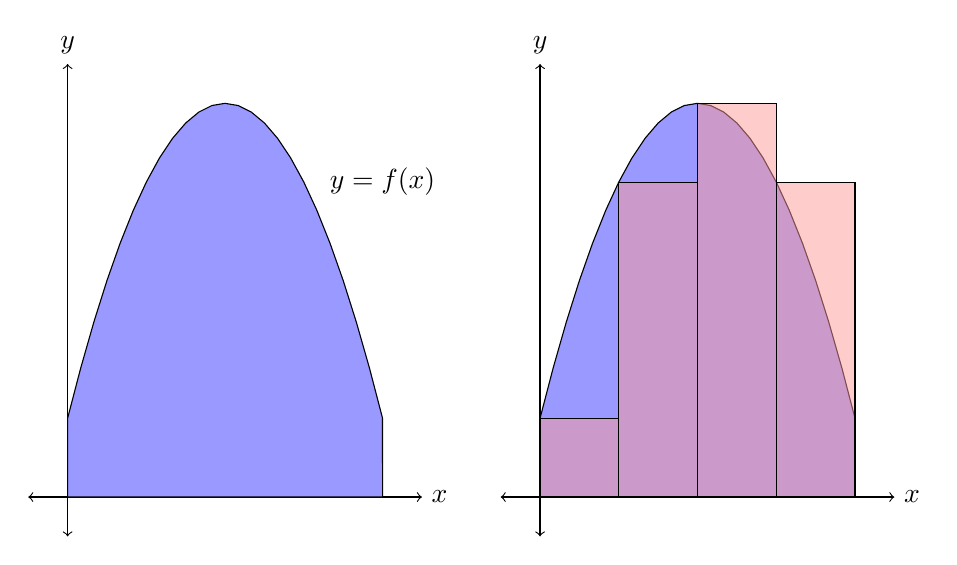
\begin{tikzpicture}[domain = 0:4]
\draw[<->] (-0.5,0) -- (4.5,0) node [right] {$x$};
\draw[<->] (0,-0.5) -- (0,5.5) node [above] {$y$};
\filldraw[fill = blue!40!white] (0,0) -- plot (\x, {5-(\x-2)^2}) -- (4,0) -- cycle;
\node at (4, 4) {$y=f(x)$};
\begin{scope}[xshift = 6cm]
\draw[<->] (-0.5,0) -- (4.5,0) node [right] {$x$};
\draw[<->] (0,-0.5) -- (0,5.5) node [above] {$y$};
\filldraw[fill = blue!40!white] (0,0) -- plot (\x, {5-(\x-2)^2}) -- (4,0) -- cycle;
\foreach \x in {0,1,2,3}
{
	\filldraw[fill = red!40!white, fill opacity = 0.5] (\x, 0) rectangle (\x+1, {5-(\x-2)^2});
}
\end{scope}
\end{tikzpicture}
\caption{การประมาณพื้นที่ใต้เส้นโค้งด้วยผลบวกรีมัน}
\label{fig:riemannsum}
\end{figure}
\end{frame}



\begin{frame}
\begin{figure}
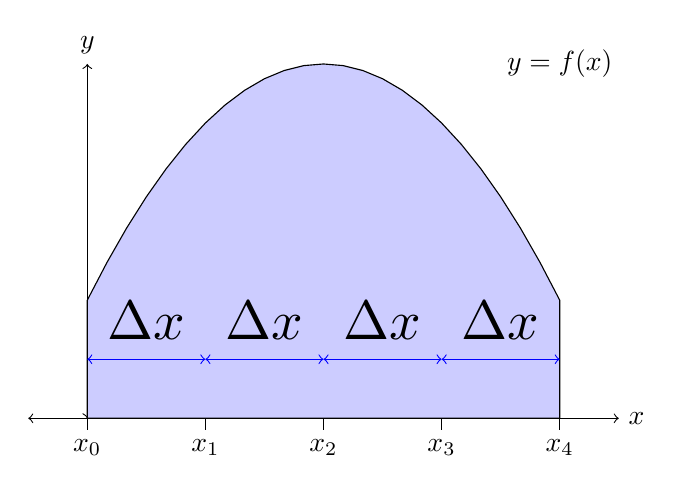
\begin{tikzpicture}[domain = 0:4, scale = 1.5]
\draw[<->] (-0.5,0) -- (4.5,0) node [right] {$x$};
\draw[<->] (0,0) -- (0,3) node [above] {$y$};
\filldraw[fill = blue!20!white] (0,0) -- plot (\x, {3-(\x-2)^2/2}) -- (4,0) -- cycle;
\node at (4, 3) {$y=f(x)$};
\foreach \x in {0,1,2,3}
{
	\draw (\x, 0) -- (\x, -0.1) node [below] {$x_\x$};
	\draw[blue, <->] (\x, 0.5) -- (\x+1, 0.5) node[pos = 0.5, above, black, scale = 2] {$\Delta x$}; 
}
\draw (4, 0) -- (4, -0.1) node [below] {$x_4$};
\end{tikzpicture}
\caption{การแบ่งช่วงย่อยที่มีความกว้างเท่ากับ $\Delta x$}
\label{fig:int_riemann_step2}
\end{figure}
\end{frame}

\begin{frame}
\begin{figure}
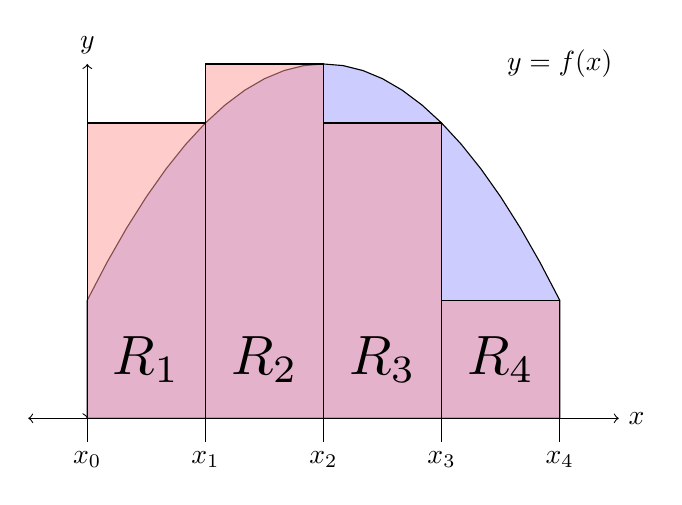
\begin{tikzpicture}[domain = 0:4, scale = 1.5]
\draw[<->] (-0.5,0) -- (4.5,0) node [right] {$x$};
\draw[<->] (0,0) -- (0,3) node [above] {$y$};
\filldraw[fill = blue!20!white] (0,0) -- plot (\x, {3-(\x-2)^2/2}) -- (4,0) -- cycle;
\node at (4, 3) {$y=f(x)$};
\foreach \x/\xp in {0/1,1/2,2/3,3/4}
{
	\draw (\x, 0) -- (\x, -0.2) node [below] {$x_\x$};
	\filldraw[fill = red!40!white, fill opacity = 0.5] (\x , 0) -- (\x, {3-(\x-1)^2/2}) --+ (1,0) -- (\x+1, 0) -- cycle;
	\node[scale = 2] at (\x+0.5, 0.5) {$R_\xp$}; 
}
\draw (4, 0) -- (4, -0.2) node [below] {$x_4$};
\end{tikzpicture}
\caption{การสร้างสี่เหลี่ยมผืนผ้า}
\label{fig:int_riemann_rect}
\end{figure}
\end{frame}

\begin{frame}{}
ถ้าเราแบ่งช่วง $[a,b]$ ออกเป็น $n$ ช่วงเท่า ๆ กัน โดยความกว้างช่วงเท่ากับ $\Delta x$ แล้วสี่เหลี่ยมผืนผ้าแต่ละรูป จะมีพื้นที่เท่ากับ 
\[ f(x_1) \Delta x, f(x_2) \Delta x, \ldots, f(x_n) \Delta x\]
เมื่อเรารวมพื้นที่ทั้งหมดเข้าด้วยกัน โดยใช้สัญลักษณ์ซิกมา จะได้พื้นที่รวมเท่ากับ
\[f(x_1) \Delta x + f(x_2) \Delta x + \ldots + f(x_n) \Delta x = \sum_{k=1}^n f(x_k) \Delta x\]
ถ้าเราต้องการให้พื้นที่นี้เข้าใกล้พื้นที่ให้เส้นโค้งมากขึ้นเรื่อย ๆ เราจะต้องเพิ่มจำนวนช่วงให้มากขึ้น โดยเราจะใช้สัญลักษณ์ลิมิตดังนี้
\[\lim_{n \rightarrow \infty} \sum_{k=1}^n f(x_k) \Delta x\]
\end{frame}


\begin{frame}
\begin{figure}
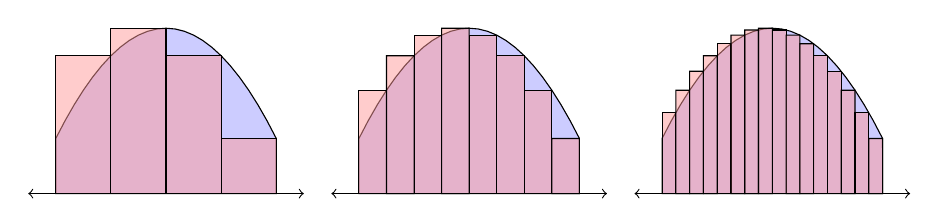
\begin{tikzpicture}[domain = 0:4, scale = 0.7]
\draw[<->] (-0.5,0) -- (4.5,0);
\filldraw[fill = blue!20!white] (0,0) -- plot (\x, {3-(\x-2)^2/2}) -- (4,0) -- cycle;
\foreach \x in {0,1,2,3}
{
	\filldraw[fill = red!40!white, fill opacity = 0.5] (\x , 0) -- (\x, {3-(\x-1)^2/2}) --+ (1,0) -- (\x+1, 0) -- cycle;
}
\begin{scope}[xshift = 5.5cm]
\draw[<->] (-0.5,0) -- (4.5,0);
\filldraw[fill = blue!20!white] (0,0) -- plot (\x, {3-(\x-2)^2/2}) -- (4,0) -- cycle;
\foreach \x in {0,0.5,1,1.5,2,2.5,3,3.5}
{
	\filldraw[fill = red!40!white, fill opacity = 0.5] (\x , 0) -- (\x, {3-(\x-1.5)^2/2}) --+ (0.5,0) -- (\x+0.5, 0) -- cycle;
}
\end{scope}
\begin{scope}[xshift = 11cm]
\draw[<->] (-0.5,0) -- (4.5,0);
\filldraw[fill = blue!20!white] (0,0) -- plot (\x, {3-(\x-2)^2/2}) -- (4,0) -- cycle;
\foreach \x in {0,0.25,0.5,0.75,...,3.75}
{
	\filldraw[fill = red!40!white, fill opacity = 0.5] (\x , 0) -- (\x, {3-(\x-1.75)^2/2}) --+ (0.25,0) -- (\x+0.25, 0) -- cycle;
}
\end{scope}
\end{tikzpicture}
\caption{เปรียบเทียบการแบ่งพื้นที่ออกเป็นช่วงที่จำนวนช่วงมากขึ้นเรื่อย ๆ}
\label{fig:int_riemann_limit}
\end{figure}
\end{frame}

\begin{frame}{}
\begin{thm}{}{}
กำหนดฟังก์ชัน $f$ ซึ่ง $f(x) \geq 0$ บนช่วง $[a,b]$ แล้วพื้นที่ใต้เส้นโค้ง $y=f(x)$ บนช่วง $[a,b]$ มีค่าประมาณเท่ากับ
\[ A \approx \lim_{n \rightarrow \infty} \sum_{k=1}^n f(x_k) \Delta x\]
โดยที่ $\Delta x = \frac{b-a}{n}$ และ $x_k = a + k\Delta x$
\end{thm}
\end{frame}

\begin{frame}[t]
\begin{ex}
จงประมาณค่าพื้นที่ใต้เส้นโค้ง $y = 2x$ ในช่วง $[0,1]$
\end{ex}
\begin{sol}
หาความกว้างช่วงได้ $\Delta x = \frac{b-a}{n} = \frac{1-0}{n} = \frac{1}{n}$

และค่า $x_k$ ได้ $x_k = a + k\Delta x = 0 + k\left(\frac{1}{n}\right) = \frac{k}{n}$

จากนั้นหาผลรวมพื้นที่สี่เหลี่ยม เมื่อแบ่งออกเป็น $n$ ช่วงย่อย
\begin{eq*}
\sum_{k=1}^n f(x_k) \Delta x &=& \sum_{k=1}^n 2\left(\frac{k}{n}\right)\left(\frac{1}{n}\right) =\frac{2}{n^2} \sum_{k=1}^n k \\
&=& \frac{2}{n^2} \left(\frac{n(n+1)}{2}\right) = \frac{n+1}{n} = 1 + \frac{1}{n}
\end{eq*}
สุดท้าย เมื่อคำนวณลิมิตจะได้ $A = \lim_{n \rightarrow \infty} 1 + \frac{1}{n} = 1$
\end{sol}
\end{frame}

\begin{frame}[t]
\begin{ex}
จงประมาณค่าพื้นที่ใต้เส้นโค้ง $y = x^2$ ในช่วง $[0,1]$
\end{ex}
\begin{sol}
หาความกว้างช่วงได้ $\Delta x = \frac{b-a}{n} = \frac{1-0}{n} = \frac{1}{n}$

และค่า $x_k$ ได้ $x_k = a + k\Delta x = 0 + k\left(\frac{1}{n}\right) = \frac{k}{n}$

จากนั้นหาผลรวมพื้นที่สี่เหลี่ยม เมื่อแบ่งออกเป็น $n$ ช่วงย่อย
\begin{eq*}
\sum_{k=1}^n f(x_k) \Delta x &=& \sum_{k=1}^n \left(\frac{k}{n}\right)^2\left(\frac{1}{n}\right) =\frac{1}{n^3} \sum_{k=1}^n k^3 \\
&=& \frac{1}{n^3} \left(\frac{n(n+1)}{2}\right)^2 = \frac{1}{3} + \frac{1}{2n} + \frac{1}{6n^2}
\end{eq*}
สุดท้าย เมื่อคำนวณลิมิตจะได้ $A = \lim_{n \rightarrow \infty} \frac{1}{3} + \frac{1}{2n} + \frac{1}{6n^2} = \frac{1}{3}$
\end{sol}
\end{frame}

\begin{frame}{นิยามปริพันธ์จำกัดเขต}
\begin{thm}{}{}
กำหนดให้ $f$ เป็นฟังก์ชันที่ต่อเนื่องบนช่วง $[a,b]$ แล้วนิยามปริพันธ์จำกัดเขตเป็นพื้นที่ใต้เส้นโค้ง นั่นคือ
\[\int_a^b f(x) \, dx = \lim_{n \to \infty} \sum_{i=1}^n f(x_n) \, \Delta x \]
\end{thm}
\end{frame}

\begin{frame}
\begin{remark}{ข้อสังเกต}
สังเกตว่า สัญลักษณ์ที่ใช้ในปริพันธ์จำกัดเขต มีที่มาจากการหาพื้นที่
\begin{itemize}
\item สัญลักษณ์ $\int$ เทียบเท่ากับ $\sum$ โดยมีที่มามาจากตัวอักษร S จากคำว่า sum เหมือนกัน
\item ขอบเขต $\int_a^b$ เทียบเท่ากับของเขต $\sum_{k=1}^{n}$ นั่นคือการคำนวณตั้งแต่ขอบเขตซ้ายสุดถึงขอบเขตขวาสุด
\item $dx$ มีความหมายเดียวกันกับ $\Delta x$ คือเป็นความกว้างช่วง โดย $dx$ แทนจำนวนที่เล็กมาก ๆ
\item $f(x) \, dx$ มีความหมายเดียวกันกับ $f(x) \Delta x$ คือการคำนวนพื้นที่สี่เหลี่ยม
\end{itemize}
\end{remark}
\end{frame}

%%%%%%%%%
\section{การหาพื้นที่ภายใต้เส้นโค้ง}
\frame{\sectionpage}
%%%%%%%%%%%

\begin{frame}
\begin{thm}{}{}
กำหนดฟังก์ชัน $f(x)$ และขอบเขต $a < b$ โดยที่ $f(x) \geq 0$ สำหรับทุกค่า $a \leq x \leq b$ แล้ว
\[ \int_a^b f(x) \, dx\]
มีค่าเท่ากับพื้นที่ที่ถูกล้อมรอบด้วยเส้นโค้ง 4 เส้น ได้แก่
\begin{itemize}
\item เส้นโค้ง $ y =f(x)$
\item แกน $x$
\item เส้นตรง $x=a$
\item เส้นตรง $x=b$
\end{itemize}
\end{thm}
\end{frame}

\begin{frame}
\begin{figure}[h!]
\centering
\begin{tikzpicture}[scale = 1.2]
\fill[fill = teal!20!white] (0,0) -- (0, 2) -- plot[smooth, domain = 0:4] (\x, {sin(\x*2 r) + 1.5}) -- (4,0) -- cycle;
\draw[<->] (-1,0)--(5,0) node[right] {$x$};
\draw[blue, smooth] plot[domain = -1:5] (\x, {sin(\x*2 r) + 1.5});
\node[blue] at (2,3) {เส้นโค้ง $y = f(x)$};
\node[teal] at (1,1) {$\int_a^b f(x) \, dx$};
\draw[red] (0,3) -- (0,-0.5) node[below left] {เส้นตรง $x=a$};
\draw[red] (4,3) -- (4,-0.5) node[below right] {เส้นตรง $x=b$};
\node at (2,-0.5) {แกน $x$};
\end{tikzpicture}
\caption{ภาพแสดงพื้นที่แรเงา ของบริเวณที่ล้อมรอบด้วยเส้นโค้ง $y=f(x)$, แกน $x$, เส้นตรง $x=a$ และเส้นตรง $x=b$}
\end{figure}
เราจะเรียกพื้นที่ดังกล่าวว่า ``พื้นที่ภายใต้เส้นโค้ง $y = f(x)$ บนช่วง $[a,b]$'' โดยเป็นที่รู้กันว่าเราหมายถึงพื้นที่เหนือแกน $x$
\end{frame}

\begin{frame}
\begin{remark}{ข้อสังเกต}
\begin{itemize}
\item เน้นย้ำว่า $f(x) \geq 0$ 
\item โดยปกติแล้ว เราจะสามารถเลือกค่า $a,b$ ได้ตามต้องการ ตราบใดที่ $f(x) \geq 0$ สำหรับทุกค่า $x$ ระหว่าง $a$ และ $b$
\item ในบางครั้ง โจทย์อาจจะไม่ได้กำหนดค่า $a,b$ มาให้ โดยจะถามในรูปแบบ
\begin{block}{}
\begin{center}
\textit{จงหาพื้นที่ระหว่างเส้นโค้ง $y = f(x)$ กับแกน $x$}
\end{center}
\end{block}
หมายความว่า โจทย์ต้องการให้เราหาค่า $a$ และ $b$ ที่ $a<b$ และ $f(a)=f(b)=0$ นั่นคือ เส้นโค้งตัดกับแกน $x$ ที่จุด $a$ และ $b$
\end{itemize}
\end{remark}
\end{frame}

\begin{frame}[t]
\begin{ex}
จงหาพื้นที่ภายใต้เส้นโค้ง $f(x) = x^2$ ที่ปิดล้อมด้วยเส้นตรง $x=1$ และ $x=3$
\end{ex}
\begin{figure}[h!]
\centering
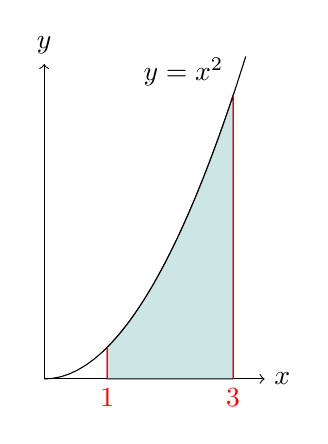
\begin{tikzpicture}[scale = 0.8]
\draw[->] (0,0) -- (3.5,0) node[right] {$x$};
\draw[->] (0,0) -- (0,5) node[above] {$y$};
\draw[domain = 0:3.2] plot (\x, {\x*\x/2});
\filldraw[fill = teal!20, domain = 1:3] (1,0) -- plot (\x, {\x*\x/2}) node[above left] {$y = x^2$} -- (3,0) -- cycle;
\draw[red] (1,0.5) -- (1,0) node[below] {1};
\draw[red] (3,4.5) -- (3,0) node[below] {3};
\end{tikzpicture}
\caption{บริเวณภายใต้เส้นโค้ง $f(x) = x^2$ สำหรับตัวอย่างที่ \theex}
\label{}
\end{figure}
\end{frame}

\begin{frame}
\begin{sol}
เนื่องจากโจทย์ให้ข้อมูลมาครบถ้วนแล้ว เราจึงสามารถหาพื้นที่ได้โดยใช้ปริพันธ์จำกัดเขตโดยตรงได้
\begin{eqnarray*}
\int_1^3 x^2 \, dx &=& \left( -\frac{1}{3}x^3 \right) \Big|_{1}^{3} \\
&=& \left( \frac{1}{3} 3^3 \right) - \left( \frac{1}{3} 1^3 \right) \\
&=& \frac{26}{3} \\
\end{eqnarray*}
\end{sol}
\end{frame}


\begin{frame}[t]
\begin{ex}
จงหาพื้นที่ภายใต้เส้นโค้ง $f(x) = \sin x$ ที่ปิดล้อมด้วยเส้นตรง $x=0$ และ $x=\frac{\pi}{2}$
\end{ex}
\begin{figure}[h!]
\centering
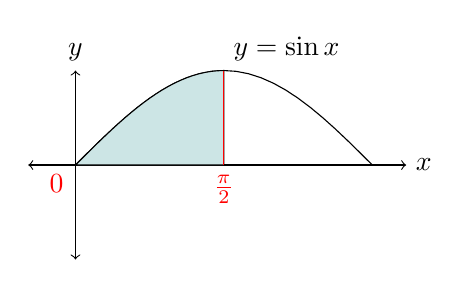
\begin{tikzpicture}[scale = 1.2]
\draw[<->] (-0.5,0) -- (3.5,0) node[right] {$x$};
\draw[<->] (0,-1) -- (0,1) node[above] {$y$};
\draw[domain = 0:3.14] plot (\x, {sin(\x r)});
\filldraw[fill = teal!20, domain = 0:1.57] (0,0) -- plot (\x, {sin(\x r)}) node[above right] {$y = \sin x$} -- (1.57,0) -- cycle;
\node[red] at (-0.2, -0.2) {0};
\draw[red] (1.57,1) -- (1.57,0) node[below] {$\frac{\pi}{2}$};
\end{tikzpicture}
\caption{บริเวณภายใต้เส้นโค้ง $f(x) = \sin x$ สำหรับตัวอย่างที่ \theex}
\label{}
\end{figure}
\end{frame}

\begin{frame}
\begin{sol}
เนื่องจากโจทย์ให้ข้อมูลมาครบถ้วนแล้ว เราจึงสามารถหาพื้นที่ได้โดยใช้ปริพันธ์จำกัดเขตโดยตรงได้
\begin{eqnarray*}
\int_0^{\pi/2} \sin x\, dx &=& (-\cos x) \Big|_{0}^{\pi/2} \\
&=& \left(-\cos \frac{\pi}{2}\right) - (-\cos 0) \\
&=& 0 + 1 \\
&=& 1
\end{eqnarray*}
\end{sol}
\end{frame}


\begin{frame}[t]
\begin{ex}
จงหาพื้นที่ภายใต้เส้นโค้ง $f(x) = 6x-3x^2$ ที่อยู่เหนือแกน $x$
\end{ex}
\begin{figure}[h!]
\centering
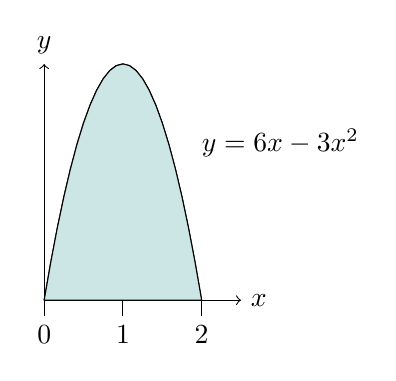
\begin{tikzpicture}[domain = 0:2]
\draw[->] (0,0) -- (2.5,0) node[right] {$x$};
\draw[->] (0,0) -- (0,3) node[above] {$y$};
\draw plot (\x, {6*\x - (3*\x*\x)});
\filldraw[fill = teal!20] plot (\x, {6*\x - (3*\x*\x)}) -- cycle;
\foreach \x in {0,1,2} 
{
\draw (\x, 0) --+ (0, -0.2) node[below] {\x};
}
\node at (3,2) {$y = 6x-3x^2$};
\end{tikzpicture}
\caption{บริเวณภายใต้เส้นโค้งสำหรับตัวอย่างที่ \theex}
\end{figure}
\end{frame}

\begin{frame}[t]
\begin{sol}
เนื่องจากโจทย์ไม่ได้กำหนดขอบเขต $[a,b]$ มาให้โดยตรง เราจึงต้องคำนวณขอบเขตจากเงื่อนไขที่กำหนดให้ ในที่นี้เงื่อนไขคือเส้นโค้งอยู่เหนือแกน $x$ นั่นคือ
\begin{eq*}
f(x) = 6x-3x^2 &>& 0 \\
3x(2-x) &>& 0 \\
3x(x-2) &<& 0 \mathnote{คูณสมการด้วยค่าลบ จึงต้องกลับเครื่องหมายอสมการ} \\
\end{eq*}

เนื่องจากรากของฟังก์ชันคือ $x=0$ และ $x=2$ เราทราบว่าฟังก์ชัน $f(x)$ จะให้ค่าลบเมื่อ $x$ อยู่ระหว่างรากทั้งสอง นั่นคืออสมการจะเป็นจริงเมื่อ  $x$ อยู่ในช่วง $[0,2]$ ทำให้เราได้ขอบเขต $[a,b] = [0,2]$ จากนั้นทำการคำนวณปริพันธ์ได้ดังนี้

\begin{eqnarray*}
\int_0^2 (6x-3x^2) \, dx &=& \left( 3x^2 - x^3\right) \Big|_{0}^{2} \\
&=& (3(2)^2 - 2^3) - (3(0)^2 - 0^3) = 12-8 = 4
\end{eqnarray*}
\end{sol}
\end{frame}

\begin{frame}[t]
\frametitle{หมายเหตุ}

\begin{columns}
\begin{column}{0.4\textwidth}
1. ค่าของปริพันธ์ติดลบได้ ถ้ากราฟอยู่ใต้แกน $x$ เช่น
\begin{slide}
\begin{eq*}
&&\int_0^2 (3x^2-6x) \, dx \\
&=& (x^3-3x^2) \Big|_{x=0}^{x=2} \\
&=& (2^3 -3(2)^2) - (0^3 - 3(0)^2) \\
&=& -4 
\end{eq*}
เราสามารถอธิบายได้ว่า พื้นที่ระหว่างแกน $x$ และเส้นโค้งมีค่าเท่ากับ 4 โดยที่เส้นโค้งอยู่ใต้แกน $x$
\end{slide}
\end{column}
\begin{column}{0.5\textwidth}
\centering
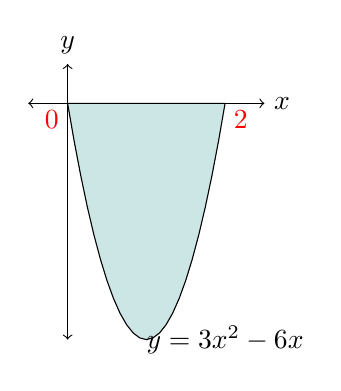
\begin{tikzpicture}
\draw[<->] (-0.5,0) -- (2.5,0) node[right] {$x$};
\draw[<->] (0,-3) -- (0,0.5) node[above] {$y$};
\filldraw[fill = teal!20, draw = black, domain = 0:2] (0,0) -- plot (\x, {3*\x*\x - 6*\x)}) -- (2,0) -- cycle;
\node at (2,-3) {$y = 3x^2-6x$};
\node[red] at (-0.2, -0.2) {0};
\node[red] at (2.2, -0.2) {2};
\end{tikzpicture}
\captionof{figure}{บริเวณใต้แกน $x$ และเหนือเส้นโค้ง $f(x) = 3x^2-6x$}
\end{column}
\end{columns}
\end{frame}

\begin{frame}[t]
\frametitle{หมายเหตุ}
2. ไม่จำเป็นต้องใส่ตัวเลขที่น้อยกว่าไว้ข้างล่าง และใส่ตัวเลขที่มากกว่าไว้ข้างบน จะใส่ตัวเลขอย่างไรก็ได้
\begin{slide}
แต่ถ้าการจะหาพื้นที่นั้นเราจำเป็นต้องใส่ตัวเลขที่น้อยกว่าไว้ด้านล่าง
\[\int_{\red{2}}^{\blue{0}} 3x^2-6x \, dx = (x^3-3x^2) \Big|_{\red{2}}^{\blue{0}} = (\blue{0}^3-3(\blue{0})^2) - (\red{2}^3 -3(\red{2}^2)) = 4 \]

โดยใช้สมบัติที่ได้ศึกษามาแล้วดังต่อไปนี้
\begin{block}{}
\[ \int_a^b f(x) \, dx = -\int_b^a f(x) \, dx\]
\end{block}
\end{slide}
\end{frame}

\begin{frame}[t]
\frametitle{หมายเหตุ}
3. พิจารณาปริพันธ์จำกัดเขตต่อไปนี้
\[\int_0^2 x^2-3x + 2 \, dx\]

\begin{figure}[h!]
\centering
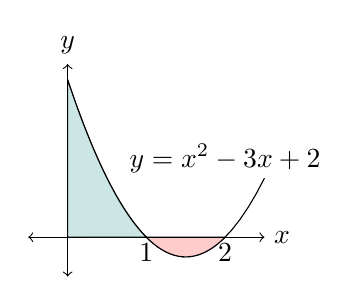
\begin{tikzpicture}
\draw[<->] (-0.5,0) -- (2.5,0) node[right] {$x$};
\draw[<->] (0,-0.5) -- (0,2.2) node[above] {$y$};
\draw[domain = 0:2.5] plot (\x, {\x*\x - 3*\x + 2});
\filldraw[fill = teal!20, draw = black, domain = 0:1] (0,0) -- plot (\x, {\x*\x - 3*\x + 2}) -- cycle;
\filldraw[fill = red!20, draw = black, domain = 1:2] (1,0) -- plot (\x, {\x*\x - 3*\x + 2}) -- cycle;
\node at (1, -0.2) {1};
\node at (2, -0.2) {2};
\node at (2,1) {$y = x^2-3x+2$};
\end{tikzpicture}
\caption{เส้นโค้งที่มีส่วนที่อยู่เหนือแกน $x$ และใต้แกน $x$}
\end{figure}
\end{frame}

\begin{frame}[t]
ถ้าเราคำนวณตั้งแต่ $x=0$ ไปถึง $x=2$ จะได้
\begin{slide}
\begin{eqnarray*}
\int_0^2 x^2-3x + 2 \, dx &=& \left(\frac{1}{3}x^3 - \frac{3}{2}x^2 + 2x\right) \Big|_0^2 \\
&=& \frac{2}{3}
\end{eqnarray*}

แต่ถ้าคำนวณแยกกันจะได้
\[ \int_0^1 x^2-3x + 2 \, dx = \blue{\frac{5}{6}} \]

และ
\[ \int_1^2 x^2-3x + 2 \, dx = \red{-\frac{1}{6}} \]

ฉะนั้น การจะหาพื้นที่ที่ถูกต้องนั้น จำเป็นที่จะต้องหาพื้นที่ระหว่างจุดตัดแกน $x$ และไม่รวมพื้นที่ที่เป็นบวกและลบเข้าด้วยกัน
\end{slide}
\end{frame}


%%%%%%%%%
\section{การหาพื้นที่ระหว่างเส้นโค้ง}
\frame{\sectionpage}
%%%%%%%%%%%

\begin{frame}
พิจารณาพื้นที่ของบริเวณที่แรเงาดังต่อไปนี้

\begin{figure}[h!]
\centering
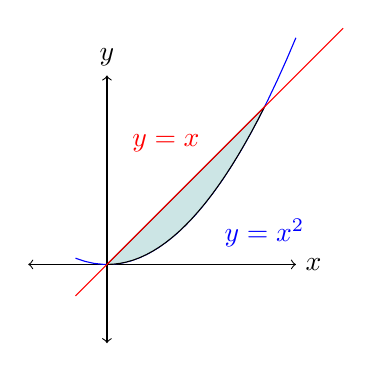
\begin{tikzpicture}[scale = 2]
\draw[<->] (-0.5,0) -- (1.2,0) node[right] {$x$};
\draw[<->] (0,-0.5) -- (0,1.2) node[above] {$y$};
\draw[blue, domain = -0.2:1.2] plot (\x, {\x*\x});
\filldraw[fill = teal!20, draw = black, domain = 0:1] (0,0) -- plot (\x, {\x*\x}) -- cycle;
\draw[red] (-0.2,-0.2) -- (1.5,1.5) node[midway, above left] {$y=x$};
\node[blue] at (1,0.2) {$y = x^2$};
\end{tikzpicture}
\caption{บริเวณระหว่างเส้นโค้ง $y=x$ และ $y=x^2$}
\end{figure}

ถ้าเราใช้แค่เครื่องมือที่มีอยู่อย่างเดียว คือ การหาพื้นที่ภายใต้เส้นโค้ง เราจะสามารถหาพื้นที่ในภาพได้อย่างไร? \pa
\end{frame}

\begin{frame}
\begin{figure}[h!]
\centering
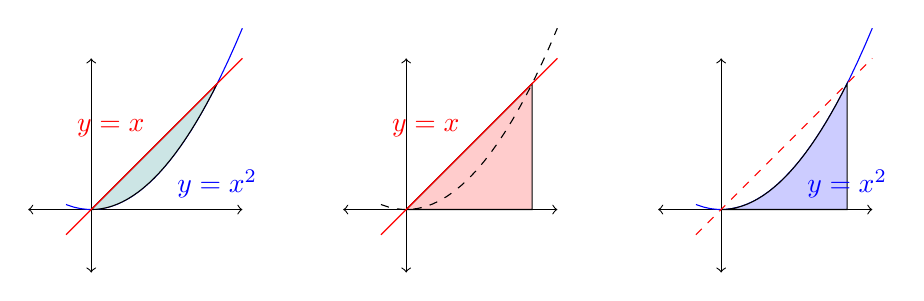
\begin{tikzpicture}[scale = 1.6]
\draw[<->] (-0.5,0) -- (1.2,0);
\draw[<->] (0,-0.5) -- (0,1.2);
\draw[blue, domain = -0.2:1.2] plot (\x, {\x*\x});
\filldraw[fill = teal!20, domain = 0:1] (0,0) -- plot (\x, {\x*\x}) -- cycle;
\draw[red] (-0.2,-0.2) -- (1.2,1.2) node[midway, above left] {$y=x$};
\node[blue] at (1,0.2) {$y = x^2$};
\begin{scope}[xshift = 2.5cm]
\draw[<->] (-0.5,0) -- (1.2,0);
\draw[<->] (0,-0.5) -- (0,1.2);
\filldraw[fill = red!20] (0,0) -- (1,1) -- (1,0) -- cycle;
\draw[dashed, domain = -0.2:1.2] plot (\x, {\x*\x});
\draw[red] (-0.2,-0.2) -- (1.2,1.2) node[midway, above left] {$y=x$};
\end{scope}
\begin{scope}[xshift = 5cm]
\draw[<->] (-0.5,0) -- (1.2,0);
\draw[<->] (0,-0.5) -- (0,1.2);
\draw[blue, domain = -0.2:1.2] plot (\x, {\x*\x});
\filldraw[fill = blue!20, domain = 0:1] (0,0) -- plot (\x, {\x*\x}) -- (1,0) -- cycle;
\node[blue] at (1,0.2) {$y = x^2$};
\draw[dashed, red] (-0.2,-0.2) -- (1.2,1.2);
\end{scope}
\end{tikzpicture}
\caption{ความสัมพันธ์ระหว่างบริเวณระหว่างเส้นโค้ง และบริเวณใต้เส้นโค้ง}
\label{fig:int_area_proof}
\end{figure}

กำหนดให้ $\green{A}$ เป็นพื้นที่ระหว่างเส้นโค้งทั้งสอง, $\red{A_1}$ เป็นพื้นที่ใต้เส้นโค้ง $y=x$ และ $\blue{A_2}$ เป็นพื้นที่ใต้เส้นโค้ง $y = x^2$ และ  จาก\figref{fig:int_area_proof} จะได้ว่า

\[ \green{A} = \red{A_1} - \blue{A_2}\]
\end{frame}

\begin{frame}
สมมติว่าเส้นโค้งที่อยู่เหนือกว่าเป็น $y = g(x)$ และเส้นโค้งที่อยู่ต่ำกว่าเป็น $y = f(x)$ \pa จะได้ว่าพื้นที่ระหว่างเส้นโค้งทั้งสอง ที่ถูกปิดล้อมด้วยเส้นตรง $x=a$ และ $x=b$ \pa มีค่าเท่ากับ 
\[ \int_a^b g(x) \, dx- \int_a^b f(x) \, dx\]

\pa ซึ่งเราใช้สมบัติของปริพันธ์จำกัดเขตเพื่อรวมให้เป็นปริพันธ์เดียวกันได้เป็น \pa
\[ \iii{a}{b}{g(x)} - \iii{a}{b}{f(x)} \pa = \iii{a}{b}{g(x) - f(x)} \]
\end{frame}

\begin{frame}
\frametitle{พื้นที่ของบริเวณระหว่างเส้นโค้ง}
เราสามารถสรุปเป็นทฤษฎีบทได้ดังนี้
\begin{thm}{}{}
กำหนดฟังก์ชัน $f(x)$ และ $g(x)$ \pa และค่าคงตัว $a, b$ \pa ที่มีสมบัติว่าเส้นโค้ง $g(x)$ อยู่เหนือเส้นโค้ง $f(x)$ ในช่วง $[a,b]$

แล้วพื้นที่ระหว่างเส้นโค้ง $y = f(x)$ และ $y = g(x)$ เท่ากับ \pa
\begin{equation}
\iii{a}{b}{(g(x) - f(x))}
\end{equation}
\end{thm}

เรากล่าวว่าเส้นโค้ง $g(x)$ อยู่เหนือเส้นโค้ง $f(x)$ ในช่วง $[a,b]$ \pa ก็ต่อเมื่อ $g(x) \geq f(x)$ สำหรับทุกค่า $x$ ในช่วง $[a,b]$
\end{frame}

\begin{frame}
\begin{figure}[h!]
\centering
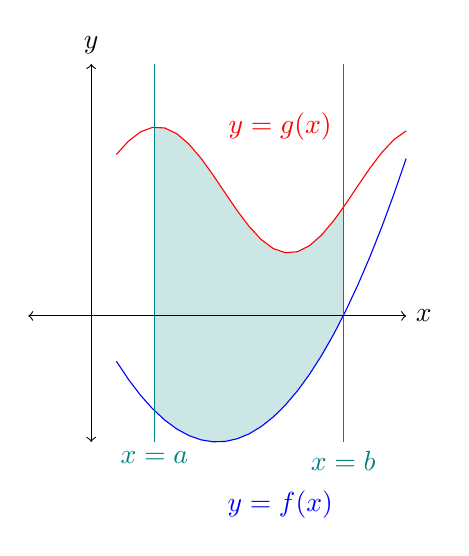
\begin{tikzpicture}[scale = 1.6]
\fill[fill = teal!20, domain = 0.5:2] (0.5,{sin(0.5 r)}) -- plot (\x, {1+sin(3*\x r)/2}) -- plot ({2.5-\x}, {(2.5-\x)*(0.5-\x)}) -- (0.5, -0.75) -- cycle;
\draw[red, domain = 0.2:2.5] plot (\x, {1+sin(3*\x r)/2});
\draw[blue, domain = 0.2:2.5] plot (\x, {\x*\x-2*\x});
\node[red] at (1.5,1.5) {$y = g(x)$};
\node[blue] at (1.5,-1.5) {$y = f(x)$};
\draw[teal] (0.5,2) -- (0.5,-1) node[below] {$x=a$};
\draw[teal] (2,2) -- (2,-1) node[below] {$x=b$};
\draw[<->] (-0.5,0) -- (2.5,0) node[right] {$x$};
\draw[<->] (0,-1) -- (0,2) node[above] {$y$};
\end{tikzpicture}
\caption{ภาพแสดงบริเวณระหว่างเส้นโค้ง $y=f(x)$ และ $y=g(x)$ ในช่วง $[a,b]$}
\end{figure}
\end{frame}


\begin{frame}
\begin{figure}[h!]
\centering
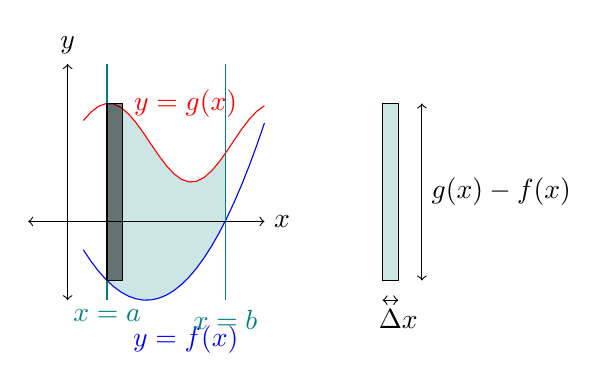
\begin{tikzpicture}
\fill[fill = teal!20, domain = 0.5:2] (0.5,{sin(0.5 r)}) -- plot (\x, {1+sin(3*\x r)/2}) -- plot ({2.5-\x}, {(2.5-\x)*(0.5-\x)}) -- (0.5, -0.75) -- cycle;
\draw[red, domain = 0.2:2.5] plot (\x, {1+sin(3*\x r)/2});
\draw[blue, domain = 0.2:2.5] plot (\x, {\x*\x-2*\x});
\node[red] at (1.5,1.5) {$y = g(x)$};
\node[blue] at (1.5,-1.5) {$y = f(x)$};
\draw[teal] (0.5,2) -- (0.5,-1) node[below] {$x=a$};
\draw[teal] (2,2) -- (2,-1) node[below] {$x=b$};
\draw[<->] (-0.5,0) -- (2.5,0) node[right] {$x$};
\draw[<->] (0,-1) -- (0,2) node[above] {$y$};
\filldraw[fill opacity = 0.5] (0.5, {1+sin(1.5 r)/2}) rectangle (0.7, -0.75);
\begin{scope}[xshift = 4cm]
\filldraw[fill = teal!20, draw = black] (0, {1+sin(1.5 r)/2}) rectangle (0.2, -0.75);
\draw[<->] (0.5, {1+sin(1.5 r)/2}) -- (0.5, -0.75) node[midway, right] {$g(x) - f(x)$};
\draw[<->] (0, -1) -- (0.2, -1) node[below] {$\Delta x$};
\end{scope}
\end{tikzpicture}
\caption{ภาพแสดงบริเวณระหว่างเส้นโค้ง $y=f(x)$ และ $y=g(x)$ ในช่วง $[a,b]$}
\end{figure}
ในมุมมองของนิยามปริพันธ์จำกัดเขต เราได้แบ่งบริเวณออกเป็นสี่เหลี่ยมผืนผ้าที่มีความสูงเท่ากับ $g(x) - f(x)$ และเนื่องจากเราหาปริพันธ์จาก  $x=a$ ถึง $x=b$ ดังนั้นปริพันธ์ที่เราต้องการจึงอยู่ในรูป $\int_a^b g(x) - f(x) \, dx$
\end{frame}



\begin{frame}[t]
\begin{ex}
จงเขียนปริพันธ์ที่ใช้หาพื้นที่บริเวณต่อไปนี้
\begin{figure}[h!]
\centering
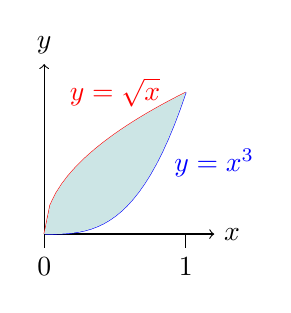
\begin{tikzpicture}[domain = 0:1, scale = 1.8]
\draw[->] (0,0)--(1.2,0) node[right]{$x$};
\draw[->] (0,0)--(0,1.2) node[above]{$y$};
\draw[red] plot (\x, {sqrt(\x)});
\draw[blue] plot (\x, {\x^3});
\fill[teal!20] plot (\x, {sqrt(\x)}) -- plot ({1-\x},{(1-\x)^3});
\node[red] at (0.5, 1) {$y = \sqrt{x}$};
\node[blue] at (1.2, 0.5) {$y = x^3$};
\foreach \x in {0,1}
{
\draw (\x,0) --+ (0, -0.1) node[below] {\x};
}
\end{tikzpicture}
\caption{ภาพสำหรับตัวอย่างที่ \theex}
\end{figure}
\end{ex}
\begin{sol}
\[ \int_0^1 \red{\sqrt{x}} - \blue{x^3} \, dx \]
\end{sol}
\end{frame}


\begin{frame}[t]
\begin{ex}
จงเขียนปริพันธ์ที่ใช้หาพื้นที่บริเวณต่อไปนี้
\begin{figure}[h!]
\centering
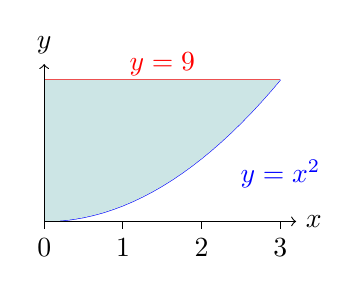
\begin{tikzpicture}[domain = 0:3, yscale = 0.2]
\draw[red] plot (\x, 9);
\draw[blue] plot (\x, {\x^2});
\fill[teal!20] plot (\x, 9) -- plot ({3-\x},{(3-\x)^2});
\node[red] at (1.5, 10) {$y = 9$};
\node[blue] at (3, 3) {$y = x^2$};
\foreach \x in {0,1,2,3}
{
\draw (\x,0) --+ (0, -0.5) node[below] {\x};
}
\draw[->] (0,0)--(3.2,0) node[right]{$x$};
\draw[->] (0,0)--(0,10) node[above]{$y$};
\end{tikzpicture}
\caption{ภาพสำหรับตัวอย่างที่ \theex}
\end{figure}
\end{ex}
\begin{sol}
\[ \int_0^3 \red{9} - \blue{x^2} \, dx \]
\end{sol}
\end{frame}


\begin{frame}[t]
\begin{ex}
จงเขียนปริพันธ์ที่ใช้หาพื้นที่บริเวณต่อไปนี้
\begin{figure}[h!]
\centering
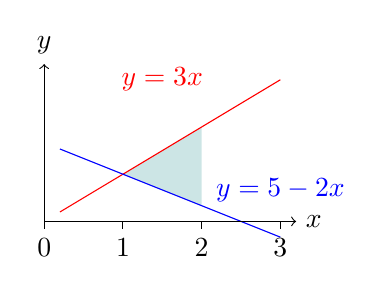
\begin{tikzpicture}[domain = 0.2:3, yscale = 0.2]
\fill[teal!20] plot (1,3) -- (2,6) -- (2,1) -- cycle;
\draw[red] plot (\x, {3*\x});
\draw[blue] plot (\x, {5-2*\x});
\node[red] at (1.5, 9) {$y = 3x$};
\node[blue] at (3, 2) {$y = 5-2x$};
\foreach \x in {0,1,2,3}
{
\draw (\x,0) --+ (0, -0.5) node[below] {\x};
}
\draw[->] (0,0)--(3.2,0) node[right]{$x$};
\draw[->] (0,0)--(0,10) node[above]{$y$};
\end{tikzpicture}
\caption{ภาพสำหรับตัวอย่างที่ \theex}
\end{figure}
\end{ex}
\begin{sol}
\[ \int_1^2 \red{(3x)} - \blue{(5-2x)} \, dx\]
\end{sol}
\end{frame}


\begin{frame}[t]
\begin{ex}
จงเขียนปริพันธ์ที่ใช้หาพื้นที่บริเวณต่อไปนี้
\begin{figure}[h!]
\centering
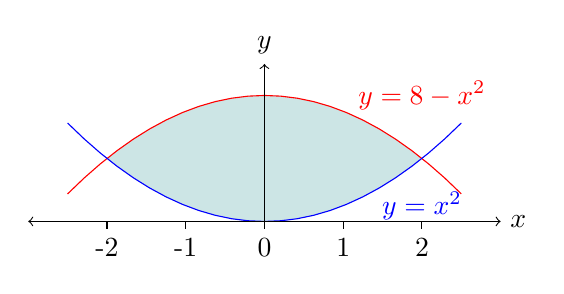
\begin{tikzpicture}[domain = -2.5:2.5, yscale = 0.2]
\fill[teal!20, domain = -2:2, smooth] plot (\x, {8-\x*\x}) -- plot ({-\x}, {\x*\x}) -- cycle;
\draw[red] plot (\x, {8-\x*\x});
\draw[blue] plot (\x, {\x*\x});
\node[red] at (2, 8) {$y = 8-x^2$};
\node[blue] at (2,1) {$y = x^2$};
\foreach \x in {-2,-1,0,1,2}
{
\draw (\x,0) --+ (0, -0.5) node[below] {\x};
}
\draw[<->] (-3,0)--(3,0) node[right]{$x$};
\draw[->] (0,0)--(0,10) node[above]{$y$};
\end{tikzpicture}
\caption{ภาพสำหรับตัวอย่างที่ \theex}
\end{figure}
\end{ex}
\begin{sol}
\[ \int_{-2}^2 \red{(8-x^2)} - \blue{(x^2)} \, dx\]
\end{sol}
\end{frame}



\begin{frame}[t]
\begin{ex}
จงหาพื้นที่ของบริเวณที่ล้อมรอบด้วยเส้นโค้ง $y = x$ และเส้นโค้ง $y = x^2$
\end{ex}
\begin{slide}
\begin{figure}[h!]
\centering
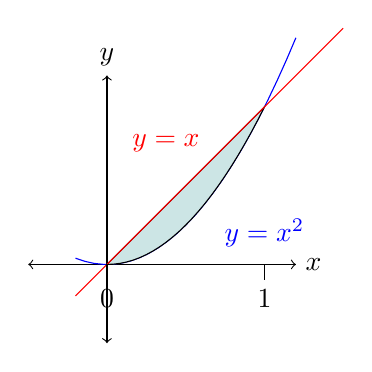
\begin{tikzpicture}[scale = 2]
\draw[<->] (-0.5,0) -- (1.2,0) node[right] {$x$};
\draw[<->] (0,-0.5) -- (0,1.2) node[above] {$y$};
\draw[blue, domain = -0.2:1.2] plot (\x, {\x*\x});
\filldraw[fill = teal!20, draw = black, domain = 0:1] (0,0) -- plot (\x, {\x*\x}) -- cycle;
\draw[red] (-0.2,-0.2) -- (1.5,1.5) node[midway, above left] {$y=x$};
\node[blue] at (1,0.2) {$y = x^2$};
\foreach \x in {0,1}
{
\draw (\x, 0) --+ (0, -0.1) node[below] {\x};
}
\end{tikzpicture}
\caption{บริเวณสำหรับตัวอย่างที่ \theex}
\end{figure}
\end{slide}
\end{frame}

\begin{frame}
\begin{sol}
เนื่องจากโจทย์ไม่ได้ให้ขอบเขต $[a,b]$ มา เราจึงต้องหาจากจุดตัดของเส้นโค้งทั้งสองด้วยการวาดกราฟ หรือการแก้สมการต่อไปนี้
\begin{eq*}
x &=& x^2 \\
x^2 - x &=& 0 \\
x(x-1) &=& 0 \\
x &=& 0, 1
\end{eq*}

ดังนั้น บริเวณที่ถูกเส้นโค้งทั้งสองล้อมรอบคือ $[a,b] = [0,1]$ และเนื่องจากในช่วง $[0,1]$ นี้ กราฟ $y=x$ อยู่เหนือกราฟ  $y=x^2$ (สังเกตจากกราฟ, จากการลองแทนค่า $x=0.5$ หรือจากการแก้อสมการ $x \leq 1 \rightarrow x^2 \leq x$) ฉะนั้นพื้นที่ของบริเวณนี้จึงมีค่าเท่ากับ

\[ \int_0^1 (x-x^2) \, dx\]
\end{sol}
\end{frame}

\begin{frame}[t]
\begin{sol} (ต่อ) สุดท้าย คำนวณปริพันธ์ได้ดังนี้
\begin{eqnarray*}
\iii{0}{1}{x - x^2} \pa &=& \frac{1}{2}x^2 - \frac{1}{3}x^3 \Big|_{x=0}^{x=1} \\ \pa
&=& \left( \frac{1}{2} 1^2 - \frac{1}{3} 1^3\right) \pa - \left( \frac{1}{2}0^2 - \frac{1}{3}0^3\right) \\ \pa
&=& \frac{1}{2} - \frac{1}{3} \\  \pa
&=& \frac{1}{6}
\end{eqnarray*}

ฉะนั้น พื้นที่ของบริเวณที่ล้อมรอบด้วยเส้นโค้ง $y = x$, เส้นโค้ง $y = x^2$ มีค่าเท่ากับ $\frac{1}{6}$
\end{sol}
\end{frame}


\begin{frame}[t]
\begin{ex}
จงหาพื้นที่ที่ล้อมรอบด้วยเส้นโค้ง $y = \cos x$, เส้นโค้ง $y = \sin x$, เส้นตรง $x=0$ และเส้นตรง $x=\frac{\pi}{4}$
\end{ex}
\begin{slide}
\begin{figure}[h!]
\centering
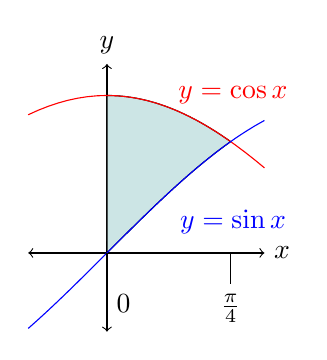
\begin{tikzpicture}[scale = 2, domain = -0.5:1]
\draw[<->] (-0.5,0) -- (1,0) node[right] {$x$};
\draw[<->] (0,-0.5) -- (0,1.2) node[above] {$y$};
\filldraw[fill = teal!20, draw = black, domain = 0:{pi/4}] (0,1) -- plot (\x, {cos(\x r)}) -- plot ({pi/4-\x},{sin((pi/4-\x) r)}) -- cycle;
\draw[red] plot (\x, {cos(\x r)});
\node[red] at (0.8,1) {$y = \cos x$};
\draw[blue] plot (\x, {sin(\x r)});
\node[blue] at (0.8,0.2) {$y = \sin x$};
\draw (0, 0) --+ (0, -0.2) node[below right] {0};
\draw ({pi/4}, 0) --+ (0, -0.2) node[below] {$\frac{\pi}{4}$};
\end{tikzpicture}
\caption{บริเวณสำหรับตัวอย่างที่ \theex}
\end{figure}
\end{slide}
\end{frame}

\begin{frame}
\begin{sol}
จากภาพเราจะเห็นว่า เส้นโค้ง $y = \cos x$ อยู่เหนือเส้นโค้ง $y = \sin x$ ในช่วง $[0,\tfrac{\pi}{4}]$ \pa ฉะนั้น พื้นที่ของบริเวณระหว่างเส้นโค้งมีค่าเท่ากับ \pa

\begin{eqnarray*}
\iii{0}{\pi/4}{\cos x - \sin x} \pa &=& (\sin x + \cos x) \Big|_{x=0}^{x=\pi/4} \\ \pa
&=& \left(\sin \frac{\pi}{4} + \cos \frac{\pi}{4} \right) \pa - (\sin 0 + \cos 0) \\ \pa
&=& \left(\frac{\sqrt{2}}{2} + \frac{\sqrt{2}}{2}\right) - (0+1) \\ \pa
&=& \sqrt{2} - 1
\end{eqnarray*}
\end{sol}
\end{frame}

\begin{frame}
\begin{remark}{ข้อสังเกต}
อันที่จริง การหาพื้นที่ระหว่างเส้นโค้ง $y=f(x)$ กับแกน $x$ ก็ใช้หลักการเดียวกัน แต่เนื่องจากแกน $x$ เป็นเส้นตรงที่มีสมการเป็น $g(x) = 0$ ดังนั้นพื้นที่จึงมีค่าเท่ากับ
\[ \int_a^b f(x) - g(x) \, dx = \int_a^b f(x) \, dx\]
\end{remark}
\end{frame}


%%%%%%%%%
\section[ทิศทางของแกน $y$]{การหาพื้นที่ระหว่างเส้นโค้ง ในทิศทางของแกน $y$}
\frame{\sectionpage}
%%%%%%%%%%%

\begin{frame}
\frametitle{พื้นที่ระหว่างเส้นโค้ง ในทิศทางของแกน $y$}
ในบางกรณี เส้นโค้งที่ให้มาอาจแบ่งเป็นเส้นที่อยู่บนและล่างไม่ได้โดยง่าย \pa แต่ถ้าเราสามารถแบ่งเป็นเส้นซ้ายกับขวาแทน เราก็จะสามารถหาปริพันธ์ได้โดยการเปลี่ยนตัวแปร และมองในแกน $y$ แทน \pa

\begin{figure}[h!]
\centering
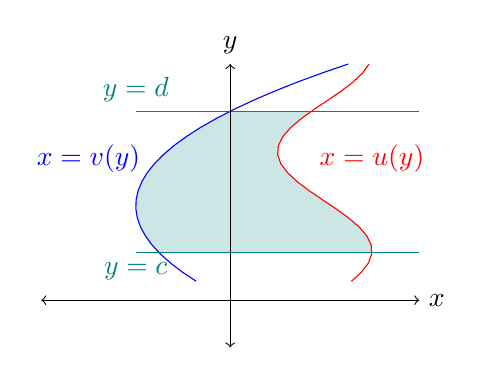
\begin{tikzpicture}[scale = 1.2]
\fill[fill = teal!20, domain = 0.5:2] ({sin(0.5 r)}, 0.5) -- plot ({1+sin(3*\x r)/2}, \x) -- plot ({(2.5-\x)*(0.5-\x)}, {2.5-\x}) -- (-0.75, 0.5) -- cycle;
\draw[red, domain = 0.2:2.5] plot ({1+sin(3*\x r)/2}, \x);
\draw[blue, domain = 0.2:2.5] plot ({\x*\x-2*\x}, \x);
\node[red] at (1.5,1.5) {$x = u(y)$};
\node[blue] at (-1.5,1.5) {$x = v(y)$};
\draw[teal] (2,0.5) -- (-1,0.5) node[below] {$y=c$};
\draw[teal] (2,2) -- (-1,2) node[above] {$y=d$};
\draw[<->] (-2,0) -- (2,0) node[right] {$x$};
\draw[<->] (0,-0.5) -- (0,2.5) node[above] {$y$};
\end{tikzpicture}
\caption{ภาพแสดงบริเวณระหว่างเส้นโค้ง $x=u(y)$ และ $x=v(y)$ ในช่วง $[c,d]$}
\end{figure}
\end{frame}

\begin{frame}
\begin{thm}{}{}
กำหนดฟังก์ชัน $x = u(y)$ และ $x = v(y)$ และค่าคงตัว $c, d$ ที่มีสมบัติว่าเส้นโค้ง $u(y)$ อยู่ด้านขวาของเส้นโค้ง $v(y)$ ในช่วง $[c,d]$

แล้วพื้นที่ระหว่างเส้นโค้ง $x = u(y)$ และ $x = v(y)$ ในช่วง $[a,b]$ มีค่าเท่ากับ
\begin{equation} 
\int_c^d ( u(y) -v(y) ) \, dy 
\end{equation}
\end{thm}

เรากล่าวว่าเส้นโค้ง $u(y)$ อยู่ด้านขวาของเส้นโค้ง $v(y)$ ในช่วง $[c,d]$ ก็ต่อเมื่อ $c<d$ และ $u(y) \geq v(y)$ สำหรับทุกค่า $c < y < d$
\end{frame}

\begin{frame}
\begin{figure}[h!]
\centering
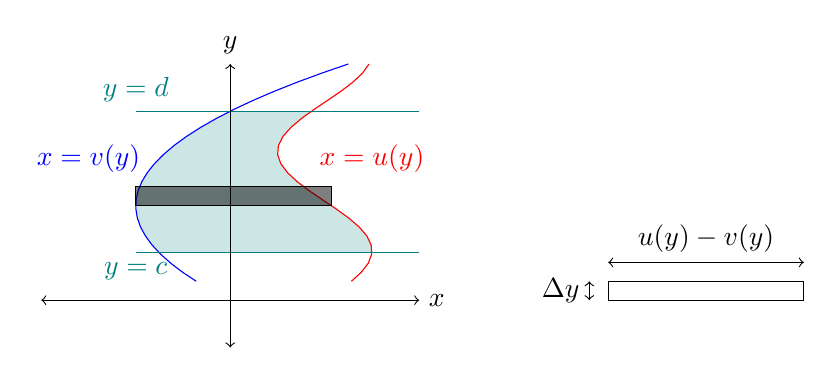
\begin{tikzpicture}[scale = 1.2]
\fill[fill = teal!20, domain = 0.5:2] plot ({1+sin(3*\x r)/2}, \x) -- plot ({(2.5-\x)*(0.5-\x)}, {2.5-\x}) -- (-0.75, 0.5) -- cycle;
\draw[red, domain = 0.2:2.5] plot ({1+sin(3*\x r)/2}, \x);
\draw[blue, domain = 0.2:2.5] plot ({\x*\x-2*\x}, \x);
\node[red] at (1.5,1.5) {$x = u(y)$};
\node[blue] at (-1.5,1.5) {$x = v(y)$};
\draw[teal] (2,0.5) -- (-1,0.5) node[below] {$y=c$};
\draw[teal] (2,2) -- (-1,2) node[above] {$y=d$};
\draw[<->] (-2,0) -- (2,0) node[right] {$x$};
\draw[<->] (0,-0.5) -- (0,2.5) node[above] {$y$};
\filldraw[fill opacity = 0.5] (-1, 1) rectangle ({1+sin(3 r)/2},1.2);
\begin{scope}[xshift = 4cm]
\draw (0,0) rectangle ({2+ sin(3 r)/2}, 0.2);
\draw[<->] (0,0.4) -- ({2+ sin(3 r)/2}, 0.4) node[midway, above] {$u(y) - v(y)$};
\draw[<->] (-0.2, 0) -- (-0.2, 0.2) node[midway, left] {$\Delta y$};
\end{scope}
\end{tikzpicture}
\caption{ภาพแสดงบริเวณระหว่างเส้นโค้ง $x=u(y)$ และ $x=v(y)$ ในช่วง $[c,d]$}
\end{figure}
ในมุมมองของปริพันธ์จำกัดเขต เราได้แบ่งบริเวณออกเป็นสี่เหลี่ยมผืนผ้าที่มีความกว้างเท่ากับ $u(y) - v(y)$ และเนื่องจากเราหาปริพันธ์จาก  $y=c$ ถึง $y=d$ ดังนั้นปริพันธ์ที่เราต้องการจึงอยู่ในรูป  $\int_c^d u(y) - v(y) \, dy$
\end{frame}


\begin{frame}[t]
\begin{ex}
จงหาพื้นที่ที่ล้อมรอบด้วยเส้นโค้ง $y  = \frac{x}{3}$, เส้นโค้ง $y= 8-x$ และแกน $x$
\end{ex}
\begin{slide}
\begin{figure}[h!]
\centering
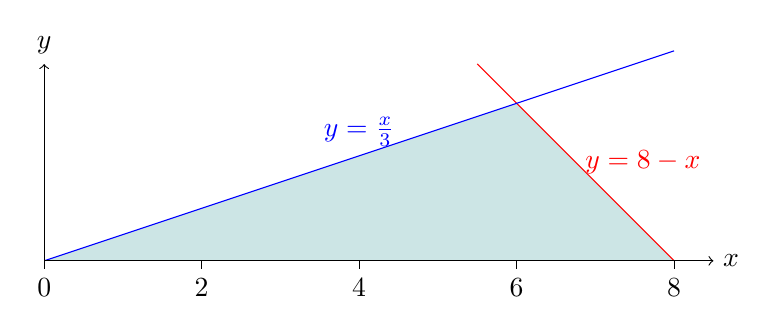
\begin{tikzpicture}
\fill[teal!20] (0,0) -- (6,2) -- (8,0) -- cycle;
\draw[red] (5.5,2.5) -- (8, 0) node[midway, right] {$y = 8-x$};
\draw[blue] (0,0) -- (8,{8/3}) node[midway, above] {$y = \frac{x}{3}$};
\foreach \x in {0,2,4,6,8}
{
\draw (\x,0) --+ (0, -0.1) node[below] {\x};
}
\draw[->] (0,0)--(8.5,0) node[right]{$x$};
\draw[->] (0,0)--(0,2.5) node[above]{$y$};
\end{tikzpicture}
\caption{ภาพสำหรับตัวอย่างที่ \theex}
\end{figure}
\end{slide}
\end{frame}

\begin{frame}
\begin{sol} แบบที่ 1 (ในทิศทางของแกน $x$): \pa เราหาจุดตัดของเส้นตรงทั้งสองเส้นได้โดยการแก้สมการ \pa
\[ \frac{x}{3} = 8-x \quad \rightarrow \pa \quad x = 6\]

\begin{figure}[h!]
\centering
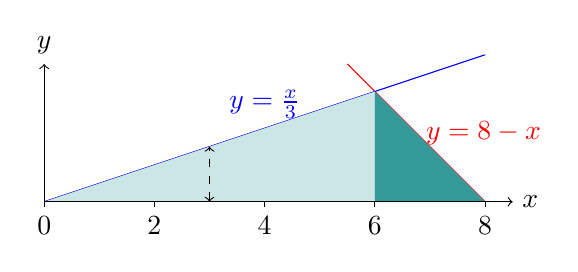
\begin{tikzpicture}[scale = 0.7]
\draw[red] (5.5,2.5) -- (8, 0) node[midway, right] {$y = 8-x$};
\draw[blue] (0,0) -- (8,{8/3}) node[midway, above] {$y = \frac{x}{3}$};
\fill[teal!20] (0,0) -- (6,2) -- (6,0) -- cycle;
\fill[teal!80] (6,0) -- (6,2) -- (8,0) -- cycle;
\foreach \x in {0,2,4,6,8}
{
\draw (\x,0) --+ (0, -0.1) node[below] {\x};
}
\draw[->] (0,0)--(8.5,0) node[right]{$x$};
\draw[->] (0,0)--(0,2.5) node[above]{$y$};
\draw[<->, dashed] (3,0) -- (3,1);
\end{tikzpicture}
\caption{การแบ่งบริเวณออกเป็นสองส่วน}
\end{figure}

จากภาพเราจะเห็นว่า มีเส้นบนอยู่สองเส้น เราจึงต้องหาปริพันธ์แยกกัน ได้เป็น
\end{sol}
\end{frame}

\begin{frame}
\begin{sol}
\begin{eqnarray*}
\iii{0}{6}{\frac{1}{3}x} \pa &=& \frac{1}{6}x^2 \Big|_{x=0}^{x=6} \\ \pa
&=& 6\\ \pa
\iii{6}{8}{8-x} \pa &=& 8x - \frac{1}{2}x^2 \Big|_{x=6}^{x=8} \\ \pa
&=& \left(8\cdot 8 - \frac{1}{2}8^2\right) - \left(8\cdot 6 - \frac{1}{2} 6^2 \right) \\ \pa
&=& (64-32) - (48 - 18) \\ \pa
&=& 2
\end{eqnarray*}
ฉะนั้น พื้นที่ทั้งหมดรวมกันได้เท่ากับ $6+2=8$
\end{sol}
\end{frame}

\begin{frame}
\begin{sol} แบบที่ 2 (ในทิศทางของแกน $y$): \pa แทนที่เราจะมองเป็นเส้นบน-ล่าง เราสามารถมองเป็นเส้นซ้าย-ขวาแทนได้ \pa

\begin{figure}[h!]
\centering
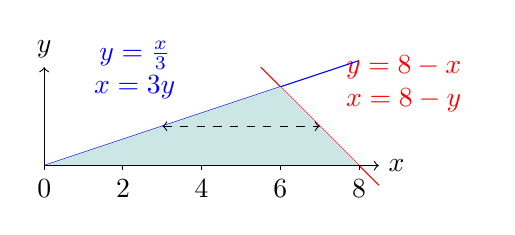
\begin{tikzpicture}[scale = 0.5]
\draw[red] (5.5,2.5) -- (8.5, -0.5) node[midway, above right] {\begin{tabular}{c} $y = 8-x$ \\ $x = 8-y$\end{tabular}};
\draw[blue] (0,0) -- (8,{8/3}) node[midway, above left] {\begin{tabular}{c}$y = \frac{x}{3}$ \\ $x = 3y$\end{tabular}};
\fill[teal!20] (0,0) -- (6,2) -- (8,0) -- cycle;
\foreach \x in {0,2,4,6,8}
{
\draw (\x,0) --+ (0, -0.1) node[below] {\x};
}
\draw[->] (0,0)--(8.5,0) node[right]{$x$};
\draw[->] (0,0)--(0,2.5) node[above]{$y$};
\draw[<->, dashed] (3,1) -- (7,1);
\end{tikzpicture}
\caption{การหาปริพันธ์ ในทิศทางแกน $y$}
\end{figure}


ทำให้เส้นตรงด้านขวา (สีน้ำเงิน) เขียนสมการใหม่ให้อยู่ในรุป $x = u(y)$ ได้เป็น \pa
\[ y = 8-x \quad \pa \rightarrow \quad x = 8-y\] \pa
และเส้นตรงด้านซ้าย (สีแดง) เขียนสมการใหม่ให้อยู่ในรูปของ $x = v(y)$ ได้เป็น \pa
\[ y = \frac{x}{3} \quad \pa \rightarrow \quad x = 3y\]
\end{sol}
\end{frame}

\begin{frame}
\begin{sol} 
จากช่วง $[0,8]$ ที่มองตามแนวแกน $x$ เราเปลี่ยนเป็นแนวแกน $y$ จะได้ช่วง $[0,2]$ แทน \pa ฉะนั้น เราหาพื้นที่ได้จากสูตร
\begin{eqnarray*}
\int_0^2 (8-y) - (3y) \, dy \pa &=& \int_0^2 8 - 4y \, dy \\ \pa
&=& 8y - 2y^2 \Big|_0^2 \\ \pa
&=& ( 8\cdot 2 - 2\cdot 2^2 ) - (8 \cdot 0 - 2 \cdot 0^2) \\ \pa
&=& 16 - 8 = 8
\end{eqnarray*}
\end{sol}
\end{frame}



\begin{frame}[t]
\begin{ex}
จงหาพื้นที่ปิดล้อมด้วยเส้นตรง $y = \frac{x}{2} - 1$ และเส้นโค้ง $x = y^2-1$
\end{ex}
\begin{slide}
\begin{figure}[h!]
\centering
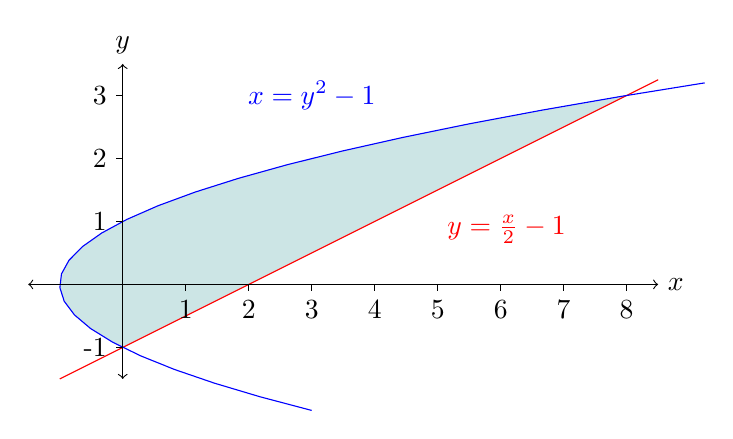
\begin{tikzpicture}[domain = -2:3.2, scale = 0.8]
\fill[teal!20, domain = -1:3] plot({\x*\x-1},\x) -- cycle;
\draw[red] (-1, -1.5) -- (8.5, 3.25) node[midway, right = 1cm] {$y = \frac{x}{2}-1$};
\draw[blue] plot({\x*\x-1},\x);
\foreach \x in {1,2,...,8}
{
\draw (\x,0) --+ (0, -0.1) node[below] {\x};
}
\foreach \y in {-1,1,2,3}
{
\draw (0,\y) --+ (-0.1, 0) node[left] {\y};
}
\draw[<->] (-1.5,0)--(8.5,0) node[right]{$x$};
\draw[<->] (0,-1.5)--(0,3.5) node[above]{$y$};
\node[blue] at (3,3) {$x = y^2-1$};
\end{tikzpicture}
\caption{บริเวณสำหรับอย่างที่ \theex}
\end{figure}

\end{slide}
\end{frame}

\begin{frame}
\begin{sol}
ขั้นแรกสุด หาจุดตัดของเส้นโค้งทั้งสองด้วยสมการ \pa
\begin{eq*}
y &=& \frac{x}{2} - 1 = \frac{y^2-1}{2} - 1 \\ \pa
y^2-2y-3 &=& 0 \\ \pa
y &=& -1, 3
\end{eq*}

เมื่อแทนค่าหา $x$ จะได้จุดตัดเป็น $(x,y) = (0, -1)$ และ $(8,3)$ \pa และเมื่อพิจารณาจากรูปของพื้นที่แล้ว เราจะหาพื้นที่โดยการหาปริพันธ์ในทิศทางของแกน $y$ \pa
แสดงว่า เราต้องเปลี่ยนฟังก์ชันให้อยู่ในรูปของ $x = h_1(x)$ และ $x = h_2(x)$ \pa จะได้ว่า
\begin{eq*}
y &=& \frac{x}{2} - 1 \\ \pa
y+1 &=& \frac{x}{2} \\ \pa
x &=& 2y+2
\end{eq*}
\end{sol}
\end{frame}

\begin{frame}
\begin{sol} (ต่อ)
เมื่อพิจารณาขอบเขตในทิศทางของแกน $y$ (นั่นคือ เมื่อลากเส้นแนวนอน) จะเห็นว่า $-1 \leq y \leq 8$ \pa ฉะนั้นพื้นที่ของรูปนี้มีค่าเท่ากับ
\begin{eq*}
&&\int_{-1}^{3} (2y+2) - (y^2-1) \, dy \\ \pa
&=& \int_{-1}^3 -y^2+2y+3 \, dy \\ \pa
&=& \left( -\frac{1}{3}y^3 + y^2 + 3y \right) \Big|_{y=-1}^{y=3} \\ \pa
&=& \left( -\frac{1}{3}3^3 + 3^2 + 3(3) \right) - \left( -\frac{1}{3}(-1)^3 + (-1)^2 + 3(-1) \right) \\ \pa
&=& 9 - \left(- \frac{5}{3} \right) = \frac{32}{3}
\end{eq*}
\end{sol}
\end{frame}



